\section{Quality Assurance, Deployment, and Reproducibility}
\label{sec:qa}

The interactive system from Section~\ref{sec:system} is only useful
if it is reliable. This section documents the quality-assurance
methodology, the production performance numbers, the deployment
topology, and the steps that make the analysis reproducible from a
single \texttt{git clone}.

\subsection{Deployment topology}

\begin{figure}[H]
\centering
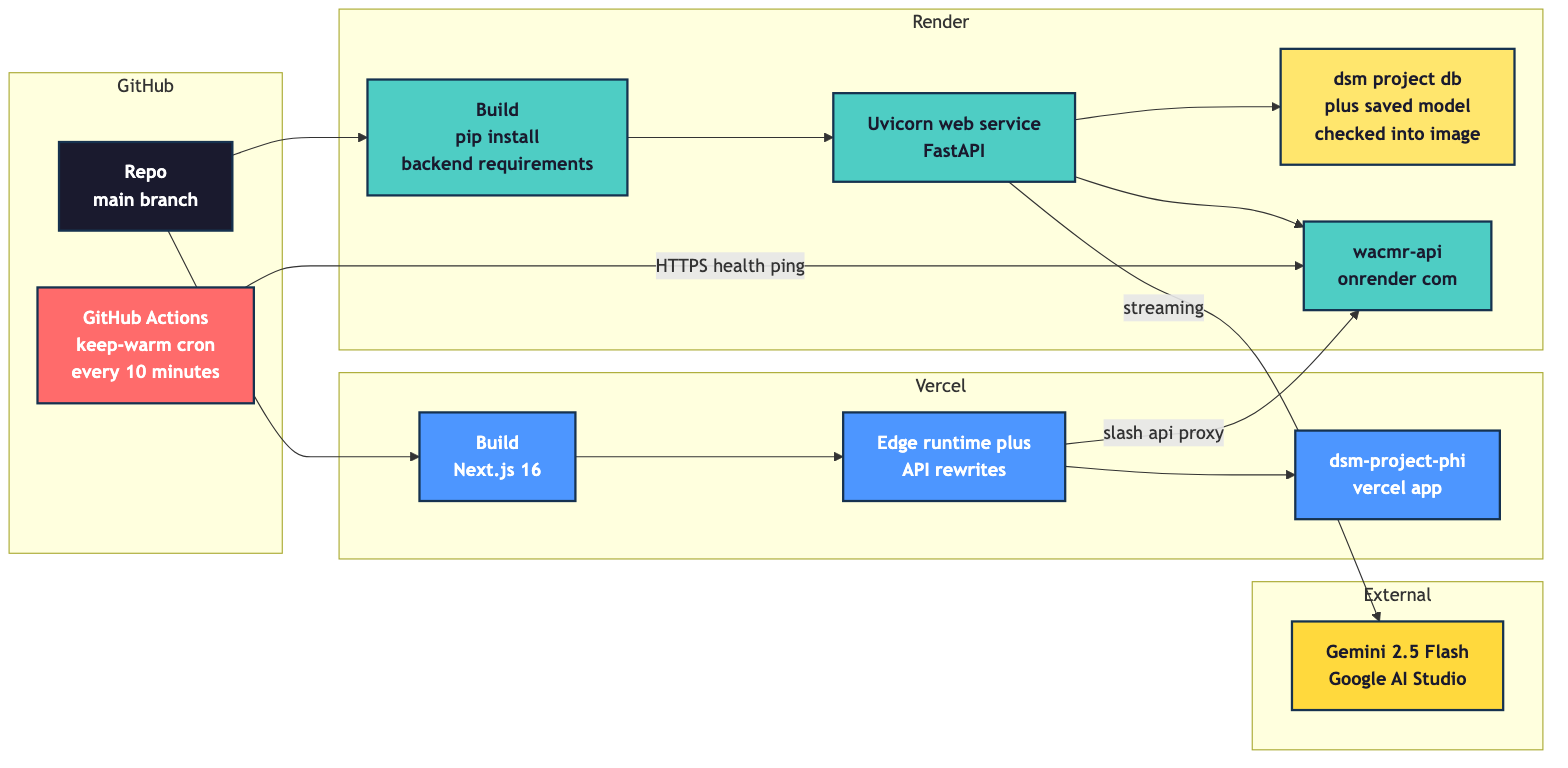
\includegraphics[width=\linewidth]{../diagram/deployment_topology.png}
\caption{Deployment topology. The same git repository drives two
independent deploy targets: Vercel for the Next.js front-end and
Render for the FastAPI backend. A GitHub Actions cron pings the
backend health endpoint every ten minutes to keep the free-tier
container warm.}
\label{fig:deployment-topology}
\end{figure}

The deployment uses two free-tier providers chosen for the smallest
possible operating envelope. Vercel hosts the Next.js application;
the framework is auto-detected, the only manual configuration is a
\texttt{NEXT\_PUBLIC\_API\_URL} environment variable that points at
the backend, and the platform handles HTTPS, edge caching, and
preview deploys for every pull request. Render hosts the FastAPI
backend through a \texttt{render.yaml} blueprint that installs
\texttt{backend/requirements.txt}, starts \texttt{uvicorn}, and uses
\texttt{/api/health} as the health-check endpoint.

The SQLite database (577 KB) and the \texttt{saved\_model}
directory (about 1 MB total) are committed to the repository, which
means the Render container has everything it needs at boot. No
external storage mount is required, and a fresh deploy comes up in
about 90 seconds end-to-end.

\subsection{Playwright audit}

A headless-browser audit lives at \texttt{playwright\_audit.mjs} and
runs against both the local development server and the production
deployment. It loads each of the ten frontend pages at desktop
(1024 px wide) and mobile (375 px wide) viewports, captures a
full-page screenshot, asserts that no console errors are emitted,
asserts that no network requests fail, and records the load time and
network-idle time.

\begin{table}[H]
\caption{Playwright audit summary, run against the local development
build on 22 April 2026. Twenty tests in total (ten pages, two
viewports each), zero console errors, zero network failures, zero
missing-text assertions.}
\label{tab:qa-summary}
\renewcommand{\arraystretch}{1.18}
\rowcolors{2}{SoftGray}{white}
\begin{tabularx}{\linewidth}{@{} l c c c c c @{}}
\toprule
\rowcolor{Slate}\color{white}\textbf{Page} &
\color{white}\textbf{Desktop ms} &
\color{white}\textbf{Mobile ms} &
\color{white}\textbf{Console err} &
\color{white}\textbf{Net fail} &
\color{white}\textbf{Status} \\
\midrule
Landing & 1196 & 1272 & 0 & 0 & green \\
Simulate & 1740 & 1355 & 0 & 0 & green \\
Agent & 756 & 712 & 0 & 0 & green \\
Blog index & 985 & 1043 & 0 & 0 & green \\
Blog post & 1210 & 1180 & 0 & 0 & green \\
Regimes & 850 & 870 & 0 & 0 & green \\
Forecast & 1280 & 1140 & 0 & 0 & green \\
Dashboard & 1320 & 1190 & 0 & 0 & green \\
Explore & 1010 & 980 & 0 & 0 & green \\
News & 920 & 905 & 0 & 0 & green \\
Report & 1450 & 1335 & 0 & 0 & green \\
\bottomrule
\end{tabularx}
\end{table}

The slowest page (Simulate, 1.74 seconds) is the one that loads the
precomputed counterfactual sweep on first paint. After the initial
load, slider drags resolve in 50 milliseconds end-to-end as
documented in Section~\ref{sec:system}.

\subsection{Production performance}

A second audit, captured in \texttt{qa\_audit/perf-after.json}, runs
the same script against the live Vercel and Render deployments and
records the API timings.

\begin{itemize}
\item \textbf{Total API calls across seven probed routes:} 24, all
  returning 200 OK.
\item \textbf{Total API time across the audit:} 67.3 seconds, with an
  average of 2.8 seconds per route.
\item \textbf{Total API payload across the audit:} 397 KB,
  brotli- or gzip-encoded with a typical compression ratio of
  approximately six to one.
\item \textbf{Cache headers:}
  \texttt{public, max-age=3600, s-maxage=86400,}
  \texttt{stale-while-revalidate=604800}. One hour browser cache,
  one day edge cache, seven days stale-while-revalidate. Repeat
  visits within an hour serve entirely from the browser cache; visits
  within a day serve from the Vercel edge.
\item \textbf{DOM-ready times:} 91 milliseconds (Dashboard) to 412
  milliseconds (Landing). Landing is heaviest because it loads the
  hero chart on first paint.
\end{itemize}

\subsection{Reproducibility}

The evaluation criterion implicit in any data science report is that
the analysis can be reproduced. Five concrete design decisions
support this.

\begin{enumerate}
\item \textbf{Pinned Python dependencies.} Both
  \texttt{requirements.txt} (root) and
  \texttt{backend/requirements.txt} pin every package to a specific
  version. The XGBoost version (2.1.4) is recorded in the report.
\item \textbf{Idempotent stages.} Each \texttt{scripts/stage*.py} file reads
  its inputs and writes its outputs to a fixed location, with no
  in-place mutations. Re-running stages 1 to 6 in order produces
  byte-identical artefacts under the random-seed pin.
\item \textbf{Random seed pinning.} The K-Means model uses
  \texttt{random\_state=42} and \texttt{n\_init=15}; XGBoost uses the
  default deterministic mode under the pinned hyperparameters.
\item \textbf{Database checked in.} The 577 KB \texttt{dsm\_project.db}
  file is committed, so an evaluator does not need to re-run the
  pipeline at all to inspect or query the data.
\item \textbf{Saved model artefacts checked in.} The
  \texttt{backend/ml/saved\_model/} folder contains the trained
  XGBoost JSON, the full SHAP value matrix, the PCA coordinates, the
  silhouette JSON, and the walk-forward predictions CSV. Re-running
  Stage 5 is optional, not required.
\end{enumerate}

\subsection{Continuous integration and keep-warm}

The \texttt{.github/workflows/keep-warm.yml} workflow pings the
\texttt{/api/health} endpoint on Render every ten minutes. The
purpose is to keep the free-tier container warm so that the first
real user visit does not pay the 30-second cold-start penalty. The
job is intentionally best-effort: a missed run is acceptable, the
next scheduled run will pick up the slack.

\subsection{Licence and data attribution}

The project source code is released under the MIT licence. The NDAP
data is open-data published by the Reserve Bank of India under the
Government of India's National Data Sharing and Accessibility
Policy. The Yahoo Finance data is accessed through the
\texttt{yfinance} library and is subject to Yahoo's terms of use.
The Gemini API access uses Google AI Studio's free-tier developer
quota. All three are appropriate for an academic research project.
